Here the goal is to present the kind of problems where persistence may prove useful and help develop reasoning needed to see other applications should they be encountered by the reader. 
Some of the examples may have more elegant solutions using a different approach.

\section{Version control systems}

Imagine a version control system is used in a repository with branching history. Each version is stored as a patch to another parent version. Naturally, one would expect to use persistent data structures for varying tasks in this scenario. A persistent binary tree could be used for example for queries of files by the last time of modification in history of that particular version.

\section{Point localization in a plane}

Given a bounded connected subset of a plane partitioned into a finite set of faces, the goal is to respond to queries asking to which face a point $p$ belongs. We limit ourselves to polygonal faces.
One special case of particular importance of this problem is finding the closest point, i.e. when the faces are Voronoi cells.

To build the data structure we will follow a general idea of line sweeping. We start by sorting vertices of all faces by the first coordinate $x$. We will continually process these vertices in the order of increasing coordinate $x$. We maintain $S$, a sorted list of edges (in a semi-persistent BST) during this processing. The list $S$ contains edges that intersect with a sweeping line parallel to the secondary axis~$y$ in order of the intersections (sorted by the second coordinate $y$).

Initially the list is empty and we set the sweeping line to intersect the first vertex.
When we start processing a new vertex we imagine moving the sweeping line along the primary axis to intersect with the new vertex. We can easily observe that the order of edges cannot change during this virtual movement. (None of the edges can intersect except at a vertex.) It will happen, however, that edges must be either removed from the list or added to the list.

We cannot store keys inside $S$ because the coordinates of intersections with the sweeping line change as it moves. To find the correct edge in $S$ one must start in the root and at each vertex calculate the intersection with the sweeping line at the given $x$ coordinate (in constant time).

We store pointers to the versions of $S$ created by processing each vertex in the plane in a sorted array. During a query, the first step is to identify which version of $S$ to use. This can be done via a binary search in versions of $S$. Then the face is identified by finding which edges in that version of $S$ are closest to the searched point.

The number of vertices will be denoted by $n$, the number of edges is thus bounded by $3n$. This follows from the partitioning being a drawing of a planar graph. Complexity is therefore \bigO{n \log n} for pre-processing and \bigO{\log n} for one query.

\begin{figure}
\def\miny{-2}
\def\maxy{5}
\def\swp #1 {\draw[loosely dashed] (#1,\miny) -- (#1,\maxy);}
\begin{center}
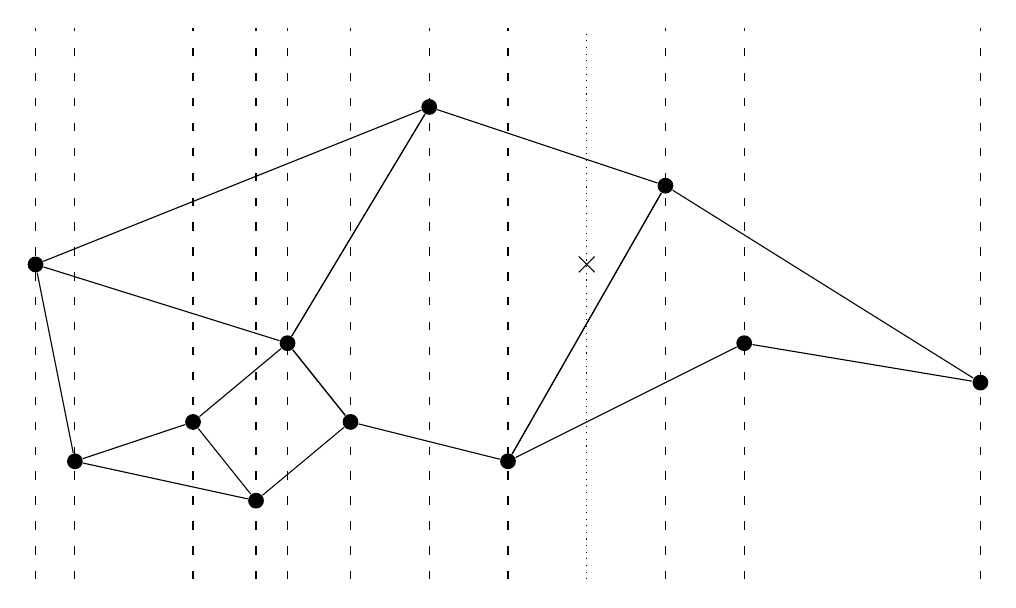
\begin{tikzpicture}[
point/.style={circle, fill=black, inner sep=0pt, minimum width=2mm},
]

\node[point] at (0.2,1) (c) {};
\node[point] at (1,0) (d) {};
\node[point] at (-0.2,-1) (a) {};
\node[point] at (-1,0) (b) {};
\node[point] at (5,3) (e) {};
\node[point] at (2,4) (f) {};
\node[point] at (-3,2) (g) {};
\node[point] at (-2.5,-0.5) (h) {};
\node[point] at (3,-0.5) (i) {};
\node[point] at (9,0.5) (j) {};
\node[point] at (6,1) (k) {};

% Rectangle:
\draw (a) -- (b) -- (c) -- (d) -- (a);

\draw (a) -- (h) -- (b);

\draw (g) -- (c);

\draw (h) -- (g) -- (f) -- (c);

\draw (c) -- (f) -- (e) -- (i) -- (d) -- (c);

\draw (i) -- (k) -- (j) -- (e) -- (i); 

\swp{-3}
\swp{-2.5}
\swp{-1}
\swp{-0.2}
\swp{0.2}
\swp{1}
\swp{2}
\swp{3}
\swp{5}
\swp{6}
\swp{9}

% Cross:
\draw (3.9,1.9) -- (4.1,2.1);
\draw (4.1,1.9) -- (3.9,2.1);
{\draw[dotted] (4,\miny) -- (4,\maxy);}
\end{tikzpicture}
\end{center}
{
    \small
    Positions of sweeping line during the run of point location algorithm are depicted as dashed lines. 
    Queried point is displayed as a cross. 
    Edges intersecting the dotted line are in the version of $S$ that will be queried.
}
\caption{Location of a point}
\end{figure}


\section{Two-dimensional prefix interval listing}

This application assumes a finite set of $n$ points in a two-dimensional plane. The request is to construct a data structure which could answer queries of the following kind: List %(the number of)
all points $(x_i,y_i)$ satisfying $x_i < \bar x$ and $ y_i \in (\underset{\bar{}}{y}, \bar y) $.

The first step in building a data structure for these queries is to sort the given points by their $x$ coordinate. Then we proceed to add all points in order of increasing $x$ coordinate into a semi-persistent binary search tree. To answer a query with the same parameters as above. We first find a version of the BST where the point added is the greatest smaller than $\bar x$ using binary search on the versions. Then we search that version of the BST and list all points in the specified interval.

With efficient implementation (as discussed in previous chapters), we get \bigO{n \log n} time to prepare the data structure, \bigO{\log n + f} time to answer a query where $f$ points are reported, and asymptotically linear memory consumption. The space requirement is an improvement over range trees \cite{range-trees}.

This data structure can be used as an alternative to range trees by looking at the difference between queries for two different $\bar x$ with the same range for $y$.

\section{Counting points inside a rectangle}

The problem can be phrased as follows: Given a set of points in a plane, efficiently find the number of points inside any rectangle $(x_1, x_2) \times (y_1, y_2)$.

Recall that we described a functional variant of binary search trees with path-copying. 
Here we realize that we can also add a field with subtree size to vertices of this BST. 
Vertices whose subtree changes in an update are copied anyway, so this extra field can be maintained without any slowdown. 

The data structure is constructed similarly to the previous section. 
All points are sorted by the $x$ coordinate in ascending order. 
Then all of them are added to the BST in order of increasing $x$ coordinate.

Counting of points inside $(x_1, x_2) \times (y_1, y_2)$ is then done by first locating correct version of the tree for $x_1$ and $x_2$. 
We then use the functional BST as a segment tree. 
To obtain the result, we determine the number of points in the tree for $x_2$ and subtract the number of points in the tree for $x_1$.

Similar geometric applications of partial persistence were investigated by Cole \cite{geometric-applications}.

\section{Binary search in a tree}

Assume we have a rooted tree $T$, a totally ordered set $S$ and a function $f: V(T) \rightarrow S$ satisfying that for every vertex $v$ and every ancestor $w$ of $v$ it holds $f(v) \leq f(w)$. 

% f is evaluated in constant time.

We would like to quickly answer a large number of queries of the following kind: For given $s \in S$ locate an ancestor $w$ of a vertex $v$ such that $f(w) \leq s$ and for every ancestor $u$ of $w$ it holds that $f(u) > s$. (There is obviously at most one suitable vertex $w$.)

We will build a data structure based on a semi-persistent binary search tree which will enable answering this kind of queries in \bigO{\log n}, where $n$ denotes the number of vertices of $T$. The first step is numbering vertices of $T$ by in-order traversal. 

We will need to efficiently answer queries for the lowest common ancestor (LCA) of two vertices. LCA of $v, w$ is such a vertex that the subtree rooted at the LCA contains both $v$ and $w$, but no of its subtrees does. LCA is thus well-defined for all pairs of vertices in rooted trees. The next step of creating the data structure is to construct a structure to answer LCA queries on the tree efficiently. This can be done efficiently in \bigO{n} via an approach described by Bender and Farach-Colton \cite{lca}, queries will use constant time.

Now we will finally start building the semi-persistent tree. We add numbers assigned to the vertices of $T$ in order of decreasing value of $f$. This involves sorting the vertices by value of $f$ and we store this sorted array for future use. Vertices in the semi-persistent tree are ordered by the assigned numbers. This is the entire preparation phase which takes \bigO{n \log n} time. The structure requires only \bigO{n} memory to store.

In order to locate vertex $w$ for given $v$ and $s$, we locate the version of the semi-persistent tree with all vertices that have value of $f$ greater than $s$. This is done by binary search in the sorted array of vertices. Once the correct version is found, we the find lower bound and the upper bound of $v$. One of these vertices must be an ancestor of $v$. This can be verified with the help of LCA structure. If both of those vertices are ancestors of $v$, we take the one further from root. 

We have now located the last ancestor of $v$ with value of $f$ greater than $s$. One of its children must be the requested vertex.

See Figure \ref{fig:cephalopoda} for an example.

Finally, we remark that other possible solution not involving persistence could utilize heavy-light decomposition.


\begin{figure}
	\footnotesize
	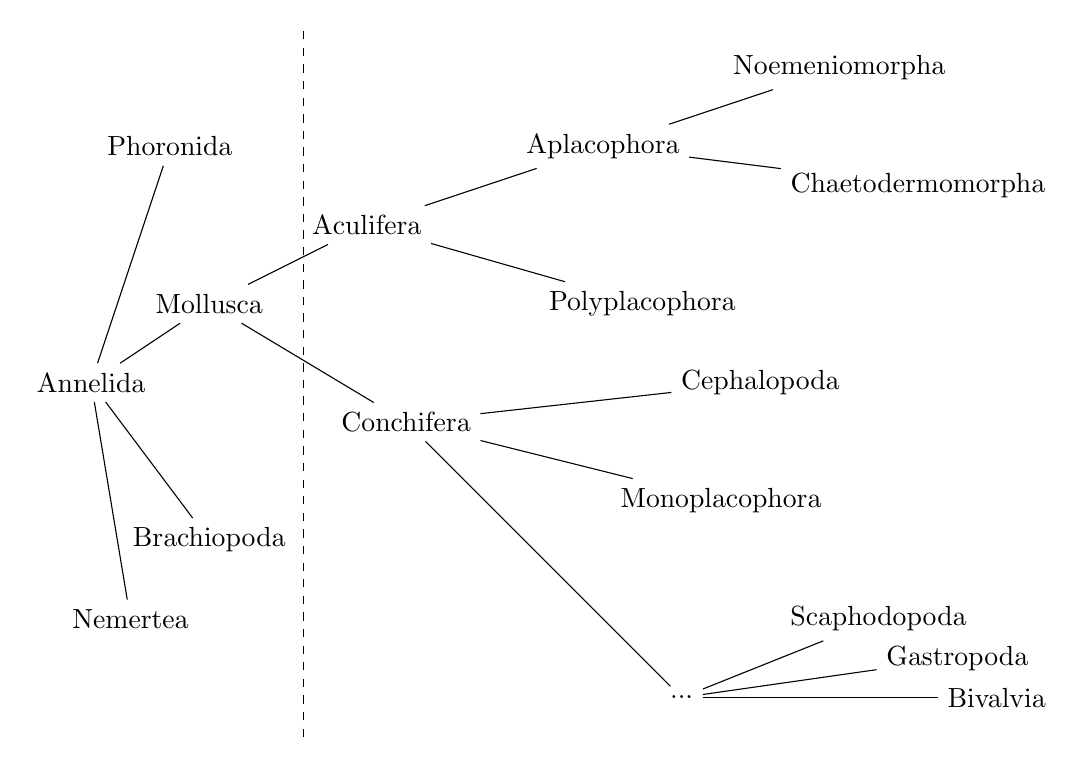
\begin{tikzpicture}
		\node at (1.5,1) (a) {Mollusca};
		\node at (3.5,2) (b) {Aculifera};
		\node at (4,-0.5) (c) {Conchifera};
		\node at (6.5,3) (d) {Aplacophora};
		\node at (7.5,-4) (e) {...};
		\node at (9.5,4) (f) {Noemeniomorpha};
		\node at (10.5,2.5) (g) {Chaetodermomorpha};
		\node at (7,1) (h) {Polyplacophora};
		\node at (8.5,0) (i) {Cephalopoda};
		\node at (8,-1.5)(j) {Monoplacophora};
		\node at (10,-3) (k) {Scaphodopoda};
		\node at (11,-3.5)(l) {Gastropoda};
		\node at (11.5,-4)(m) {Bivalvia};
		\node at (0.5,-3) (n) {Nemertea};
		\node at (1.5,-2) (o) {Brachiopoda};
		\node at (1,3) (p) {Phoronida};
		\node at (0,0) (q) {Annelida};
		
		\draw (q) -- (a);
		\draw (q) -- (n);
		\draw (q) -- (o);
		\draw (q) -- (p);
		
		\draw (a) -- (b);
		\draw (a) -- (c);
		
		\draw (b) -- (d);
		\draw (b) -- (h);
		
		\draw (d) -- (f);
		\draw (d) -- (g);
		
		\draw (c) -- (i);
		\draw (c) -- (j);
		
		\draw (c) -- (e);
		\draw (e) -- (k);
		\draw (e) -- (l);
		\draw (e) -- (m);
		
		\draw[dashed] (2.7,-4.5) -- (2.7,4.5);
	\end{tikzpicture}
	\normalsize
	\caption{Fictitious phylogenesis of Cephalopoda}
	Taxonomic units are ordered by the time of speciation (left to right) and connected by supposed ancestry. (Biological facts were heavily modified by the author.)
	Assuming a query for $v =$ \emph{Chaetodermomorpha} and $s$ represented by the dashed vertical line, \emph{Mollusca} and \emph{Phoronida} are found to be lower and upper bound in the appropriate version of the persistent tree, of which \emph{Mollusca} is found to be ancestor of $v$ through LCA. Finding LCAs of its children and $v$, it is discovered that \emph{Aculifera} is the answer.
\end{figure}

\section{Dynamic binary search in a tree}

In the previous example we considered that the tree $T$ where queries would be conducted would be static. With full persistence we can afford to add and remove vertices.

Let $m$ denote the total number of vertices added to the tree.

We will maintain a fully-persistent balanced binary search tree $P$ with vertices ordered by values of $f$. When we want to insert a vertex $z$ to $T$, we also add this vertex to the version of $P$ which was created by adding the parent of $z$. This insert will thus cost \bigO{\log m}.

A query with $s \in S$ and $v \in V(T)$ is simply answered by a search in $P$ in the version created by adding $v$ to $T$. Complexity will be \bigO{\log m}.

Deleting leaves is easy -- no actual procedure is needed. Support for deletion of non-leaf vertices $z$ from $T$ can also be added. Precisely that means that all children of $z$ become children of the parent of $z$. (For simplicity we will assume that root will never be deleted, which is a reasonable assumption as an extra root can be added.) 

Vertices are placed into a disjoint-find-union data structure (DFU) \cite{dfu} as singletons. DFU stores a system of disjoint sets and allows the following operations:

\begin{itemize}
\item {\tt Find(Vertex)} locates the representative of the set containing {\tt Vertex}.
\item {\tt Union(VertexA, VertexB)} removes sets containing {\tt VertexA} and {\tt VertexB} and adds their union to the data structure.
\end{itemize}

When a vertex is deleted, it is united with its parent in this DFU data structure. It can be seen that every component in the DFU has a unique root. When searching through $P$ instead of using values of vertices directly, we search the DFU and use vertex found as root of component in the DFU.

This clearly does not break the ordering of vertices in $P$, as there are no possible keys between those of a vertex and its parent for every version. 
 
Not to store excessively many deleted vertices in $P$ and the DFU, we rebuild the entire data structure from the latest version of $T$ when the amount of deleted vertices reaches at least half of the total amount of vertices. The cost to rebuild the tree is obviously amortized into a constant per delete.
 
Depending on the ratio between types of operations, complexity of the queries may be increased. %TODO: Is this amortized completely?

Alternatively, this problem may in addressed by adding a few extra operations to link/cut trees \cite{link-cut}.